\section{Modeling and Performance Analysis of PID Controlled BLDC Motor and Different Schemes of PWM Controlled BLDC Motor}

 Brushless DC motors are continuously earning reputation in the electronics side of things preferably in motion control applications. This DC motor has a low maintenance factor as well as it has a higher efficiency rate. On this paper of Singh Patel and Pandey presents the modeling and performance analysis of a brushless DC motors which are PID controlled. The paper also contains different schemes of brushless DC motors that are PWM controlled. According to them one of the key differences of DC motor and brushless one is that the brushless DC motor has brushes attached on its stator. 
\par
\par
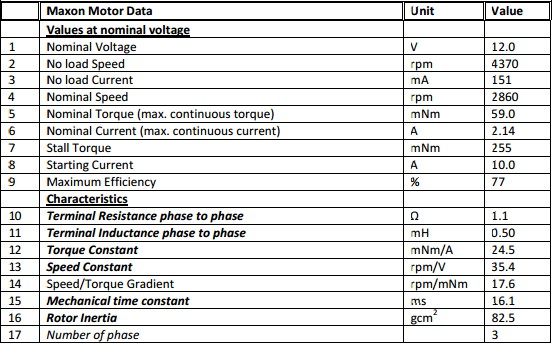
\includegraphics[width=12cm]{Table1}
\par
{\centering
  Table 1: BLDC Motor Parameters Used\par
}

\section{Autonomous Machine Vision for Off-Road Vehicles in Unstructured Fields}

Some issues that are tackled with a study relating to the machine vision are camera installation pose automatic calibration, vehicle heading estimation and field edge detection. On the research conducted by Wang, a stereo color camera was used to address the three issues mentioned. These cameras are used as sensors for perception for agricultural vehicle navigation. A problem rises whenever this camera is used and it is the difficulty of determining the camera’s pose corresponding to the vehicle frame. On the research, Wang implemented a machine vision algorithm which detects static feature points on the ground. It also tracks the three dimensional motions with regards to the vehicle. The main goal of the research is to determine the feasibility of the machine vision to find clues based on the natural visual references in an open agricultural field. To achieve this goal, a binocular stereo camera was selected, because it could provide both color information and 3D space information about a scene. (Wang, 2009).



\section{Arduino Based Photovore Robot}

The main goal of this research is to create a design of a robot which can be controlled by using light. A light sensor is going to be used so that the robot would be able to follow the light that is to be emitted. An Arduino board would also be used to implement and program the robot. The analog pins of the Arduino board are going to be used to be able to read the analog data that is acquired from the sensors. A specific set of codes as well are going to be used so that the robot would move accordingly and properly. If both sensors read about the same value, meaning the both get the same amount of light, then robot should drive straight. (Singh, 2013)



\section{Wi-Fi Remote Control Car via Mobile Device}



This project is centered on designing a Wi-Fi remote controlled car using a mobile device. In order to do this, we need a remote control that using wirelessly transmits that used RF technology, and data to the vehicle to move in any way (Hoong, 2013). The research contains an automatic mode in which the car follows the input direction of the user on the controls. The device screen of the mobile is located on the remote control so it can display the direction, distance and mode to plan on the distance and by a button. Although there would be such problems that can occur including the absence of accelerometer on this research by Hoong. 




\section{The Wireless Remote Control Car Based on Arm9}


Wi-Fi based Wireless remote control has the features of high bandwidth and rate, non-line-transmission ability, large-scale data collection and high cost-effective, and it has the capability of video monitoring, which cannot be realized with RF (Joginaidu & Marudi, 2013). This research of the group has a high significance to the development of the electronics industry. The research if more focused on controlling the car through the use of Wi-Fi module. The remote controlled car is then going to be monitored through remote PC or Laptop which also supports the Wi-Fi technology. 


\section{Summary}
